\documentclass[10pt]{article}

\usepackage[utf8]{inputenc}
\usepackage[T1]{fontenc}
\usepackage[margin=1in]{geometry}
\usepackage{authblk}
\usepackage{graphicx}
\usepackage{booktabs}
\usepackage{array}
\usepackage{longtable}
\usepackage[protrusion=true,expansion=false]{microtype}
\usepackage{xcolor}
\usepackage{amsmath}
\usepackage{natbib}
\usepackage{url}
\usepackage{xspace}
\usepackage[hidelinks]{hyperref}
\usepackage{cleveref}
\usepackage{placeins}

\setlength{\emergencystretch}{3em}
\Urlmuskip=0mu plus 1mu

\renewcommand{\Authfont}{\large\bfseries}
\renewcommand{\Affilfont}{\small\normalfont}
\setlength{\affilsep}{0.5em}

\graphicspath{{figures/generated/}}
\newcommand{\dataset}{\textsc{PT60-Candidate}\xspace}
\newcommand{\project}{\textsc{PortugueseOPD}\xspace}
\newcommand{\code}[1]{\texttt{#1}}
\newcommand{\status}[1]{\textsc{#1}}
\newcommand{\todoauthor}{\textbf{[AUTHOR INPUT NEEDED]}}
\newcommand{\resultneeded}{\textbf{[RESULT NEEDED]}}
\newcommand{\osminfra}{OSM/\allowbreak OpenInfraMap\xspace}

\title{A provenance-tracked candidate dataset for Portuguese 60~kV topology reconstruction}
\author[1]{\todoauthor}
\affil[1]{[AFFILIATION INPUT NEEDED]}
\ifdefined\PTPublicValidationOnly
\date{July 2026\\\small Scientific Data draft; public-source validation route}
\else
\date{July 2026\\\small Scientific Data draft; author review copy}
\fi

\begin{document}
\maketitle

\begin{abstract}
Open infrastructure portals often provide geospatial power-network records without explicit bus--branch connectivity, record-level provenance, or machine-readable statements of what remains inferred or unknown. We assembled \dataset, a provenance-tracked candidate dataset for Portuguese 60~kV topology reconstruction derived from E-REDES Open Data. The release workflow preserves source observations, deterministic transformations, inferred connectivity, diagnostic assumptions, proxy semantics, and missing fields as distinct states rather than collapsing them into a single network model. For the documented source snapshot, 5,334 line features and 586 relevant facility records were processed across 216 reconstruction settings. The selected release contains a 484-facility candidate multigraph, 358 retained inter-facility branch records, a 1,342-row circuit-classification ledger that also preserves downgraded outcomes, a reconstruction-sensitivity table, source and assumption manifests, public-source triangulation outputs, and staged derivative interfaces for downstream tabular and graph consumers. Technical validation covers geometry parsing, coordinate-reference handling, schema and referential checks, graph/table parity, release-contract validation, sensitivity analysis, and comparison with Portuguese 60~kV records from \osminfra. For the current snapshot, this comparison assigns 247 retained branches to strong, 104 to medium, and seven to weak public-evidence categories. These categories measure concordance with a public geospatial layer; they are not truth labels and do not yield topology precision or recall. The release is intended for reconstruction research, geospatial data integration, provenance-aware benchmarking, and dataset-engineering studies. It is not an operator-confirmed representation of the Portuguese grid, and its optional electrical and learning extensions remain diagnostic because key parameters and labels are incomplete, proxy-based, or scenario-derived.
\end{abstract}

\noindent\textbf{Keywords:} power-grid dataset; data provenance; topology reconstruction; distribution networks; technical validation; open data

\section{Background \& Summary}

Public distribution-network portals can support geospatial and data-integration studies, but the released records rarely correspond directly to an auditable bus--branch dataset. Connectivity must usually be inferred from facility locations and line geometries, while electrical parameters, switching states, and operating conditions remain incomplete or unavailable. In this setting, a reusable dataset should not only publish retained candidate connections; it should also preserve how those candidates were constructed, what evidence supports them, and which fields remain unknown or diagnostic.

\dataset was assembled to provide such a resource for a Portuguese E-REDES 60~kV layer. The release is explicitly a \emph{candidate} dataset. It does not represent an operator-confirmed connectivity model, a national Portuguese grid model, or a validated electrical operating case. Instead, it provides a provenance-tracked reconstruction product in which retained branches, downgraded circuits, release manifests, validation outputs, and downstream interface contracts remain inspectable as part of the data record.

The release contains three closely related resource types. First, it provides a core topology layer composed of retained inter-facility branches, an all-facility multigraph, and a complete circuit-classification ledger. Second, it provides validation and provenance records, including a reconstruction-sensitivity sweep, a source manifest, a public-source audit, and branch-level triangulation outputs. Third, it provides staged derivative interfaces that expose the same candidate resource to tabular, graph, benchmarking, and framework-neutral adapter consumers while preserving provenance and governance metadata.

This framing differs from a conventional engineering paper. The central contribution is the release of a documented candidate dataset and its validation boundaries, not a claim of algorithmic novelty or a demonstration of predictive superiority. Prior open-grid resources have shown the value of transparent power-system model construction from public records \citep{Medjroubi2017,Rivera2019,Horsch2018,Xiong2025,Wiese2019}. \dataset extends that tradition to a Portuguese 60~kV distribution-layer reconstruction problem while making rejected circuits, semantic status fields, and downstream release contracts explicit.

\section{Methods}

\subsection{Source datasets}

The source snapshot combines AT line geometries, AT substations, switching facilities, MT-substation context, network-characteristics tables, substation-load records, reception-capacity context, and load-diagram indices from the E-REDES Open Data Portal \citep{EREDESOpenData2026}. For the documented snapshot, the topology stage loads 586 technically relevant facilities, comprising 409 AT substations and 177 additional facilities. The same snapshot contains 5,334 valid AT line features, of which 5,323 are labeled 60~kV and 11 are labeled 130~kV in the current local build.

The release uses the portal-level license statement reported by E-REDES for distributable data artifacts. The intended dataset package therefore records the publisher attribution, portal URL, source dataset identifiers, access dates, and transformation notices separately from the repository's MIT code license. Where topology-critical API catalog responses did not repeat an explicit license field, the release policy follows the archived portal-level statement rather than inferring a different license from the omission. Final archive identifiers and the frozen snapshot date should be inserted before submission as `[DATASET DOI NEEDED]`, `[VERSIONED ARCHIVE URL NEEDED]`, and `[FROZEN SNAPSHOT DATE NEEDED]`.

\subsection{Data acquisition}

Source files are downloaded and validated through a reproducible workflow that records dataset roles, retrieval checks, and release metadata in a source manifest. The source manifest currently covers 13 datasets and is intended to accompany any public release. Geometry parsing and machine-readability checks occur before reconstruction so that parse failures become explicit blocking states rather than silent exclusions.

The acquisition scope is limited to the E-REDES AT layer represented in the documented snapshot. It does not include a verified REN transmission boundary, complete national generation, measured operating conditions, or authoritative switching-state data. These omissions are treated as scope boundaries of the dataset rather than as gaps to be silently imputed.

\subsection{Data preprocessing}

Preprocessing harmonizes source geometries, facility identifiers, and facility classes before topology inference. The workflow validates geometry type and validity, repairs parseable geometry issues where permitted by the loader, performs coordinate-reference conversions needed for endpoint and corridor calculations, and derives geometry-based quantities such as length. These transformations are recorded as derived rather than observed values.

Facilities are standardized into node candidates with associated codes, names, types, source roles, and footprint-ready geometries. Source line features are standardized into endpoint-bearing line records. Ambiguous matches and unresolved endpoints are retained as explicit states for later classification. This preprocessing stage therefore prepares line and facility inputs for reconstruction without asserting that each input line already corresponds to a valid inter-facility branch.

\subsection{Provenance model}

The release uses a field-level semantic status model so that downstream users can separate copied observations from deterministic derivations, inferred topology, and diagnostic assumptions. For an object $o$ at stage $k$, the workflow records
\begin{equation}
T_k(o)=(v,s,q,a,e),
\end{equation}
where $v$ is the value, $s$ its semantic status, $q$ a quality or confidence indicator, $a$ a source or assumption identifier, and $e$ an exclusion or blocking reason.

\begin{table}[t]
\centering
\small
\caption{Semantic statuses used in \dataset and its derivative interfaces.}
\label{tab:semantics}
\begin{tabular}{p{0.19\textwidth}p{0.71\textwidth}}
\toprule
Status & Interpretation \\
\midrule
Observed & Copied from an E-REDES record, subject to source and join quality. \\
Derived & Deterministic transformation, such as geometry length. \\
Inferred & Connectivity produced by matching, clustering, merging, or classification. \\
Source-backed & Supported by an applicable operator, standard, or catalog source. \\
Scenario-assumed & Explicit choice used only in a named diagnostic scenario. \\
Benchmark-only & Non-Portuguese reference value used only for software and interface testing. \\
Proxy & Surrogate identity, injection, capacity, dispatch, or cost semantics. \\
Missing & Intentionally unfilled; dependent readiness gates must block use. \\
\bottomrule
\end{tabular}
\end{table}

These statuses are carried into manifests and derivative interfaces so that consumers can apply explicit admissibility rules. A complete field-level data dictionary should be supplied as Supplementary Table~S1 `[DATA DICTIONARY / SUPPLEMENT TABLE NEEDED]` and a checksum-linked release manifest should be supplied as `[CHECKSUM MANIFEST REFERENCE NEEDED]`.

\subsection{Reconstruction pipeline}

Facility records are converted to circular footprints with radii of 50, 100, 250, and 500~m. Three node sets are evaluated: set A contains 409 AT substations, set B contains 484 AT substations and switching facilities, and set C contains all 586 technically relevant facilities. Each source line contributes two endpoints. When an endpoint intersects multiple footprints, the workflow resolves membership by centroid distance and records ambiguity where needed rather than forcing an unqualified assignment.

Endpoints are then clustered at 0.5, 1, 5, 10, 25, and 50~m. Union--find merging groups features into circuit candidates under geometry-only, voltage-aware, or voltage-plus-status-aware compatibility rules. Explicit conflicts block merging in the corresponding compatibility mode. Endpoint-cluster degree is then used to distinguish ordinary terminal pairs from loop, self-loop, isolated, and tap or multi-terminal patterns.

\begin{figure}[t]
  \centering
  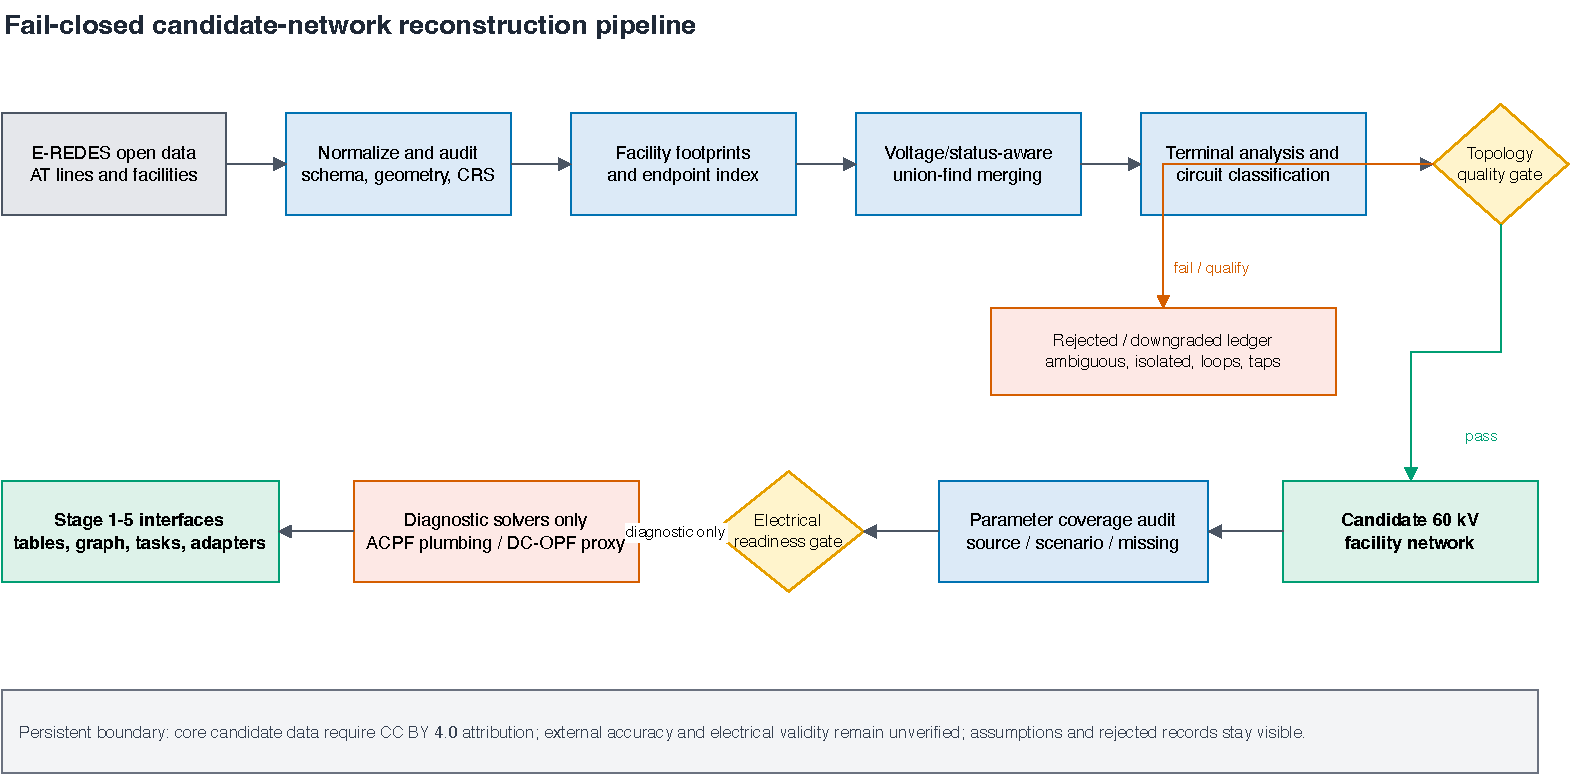
\includegraphics[width=\textwidth]{fig1_pipeline_overview.pdf}
  \caption{Dataset-generation workflow for \dataset. Blue boxes denote transformations, yellow diamonds denote gates, green boxes denote retained release artifacts, and red boxes denote diagnostic or downgraded outcomes. The diagram summarizes workflow structure and validation boundaries rather than measured performance.}
  \label{fig:pipeline}
\end{figure}

\subsection{Candidate selection}

A merged group is retained as an inter-facility candidate branch only when it has exactly two terminals, both terminals match facilities without disqualifying ambiguity, and the two facilities are distinct. Outcomes failing these conditions remain available in the circuit-classification ledger as loop, self-loop, single-facility, isolated, tap or multi-terminal, ambiguous, or otherwise downgraded records.

This selection policy is intentionally conservative. It favors explicit preservation of non-retained outcomes over optimistic retention. Mixed voltage or status conflicts, suspicious spatial matches, and unresolved facility mappings are retained as audit information instead of being absorbed into a simplified final graph.

\subsection{Parameter sweep}

The reconstruction workflow evaluates 216 settings generated by combining three facility sets, four footprint buffers, six endpoint snap thresholds, and three merge modes. The selection rule rewards retained inter-facility yield and interpretable component structure while penalizing ambiguity, explicit conflicts, suspicious matches, and the broadest thresholds. The selected release setting uses node set B, a 100~m facility buffer, a 0.5~m endpoint snap threshold, and voltage-plus-status-aware merging.

The score is a reproducible engineering rule used to choose one documented release point from the 216-setting sweep. It is not a calibrated probability of correctness and is not presented as an external optimum.

\subsection{Dataset generation}

The selected setting converts 5,334 source line features into 1,342 circuit candidates. Of these, 358 satisfy the declared inter-facility rules and are released as retained candidate branches. The remaining 984 circuit candidates are preserved as downgraded records rather than discarded. The selected all-facility GraphML preserves isolated facilities as nodes so that graph outputs remain consistent with the declared isolate policy.

The same workflow also packages derivative records: a reconstruction-sensitivity table, public-source triangulation outputs, a source audit, a source manifest, optional electrical-readiness summaries, and staged Stage~1--5 interfaces for downstream consumers. These derivative products are part of the release because they document how the candidate dataset should be interpreted and reused.

\section{Data Records}

\subsection{Repository overview}

The release is organized around a core topology package, validation and provenance records, and optional derivative interfaces. The manuscript describes the current artifact set as generated in the local repository build. A public archive should freeze these records under `[DATASET DOI NEEDED]` and `[VERSIONED ARCHIVE URL NEEDED]`, together with a release manifest, file hashes, access dates, and attribution text.

The core release should include at least the retained branch table, the circuit-classification ledger, the selected GraphML multigraph, the reconstruction-sensitivity table, the source manifest, and the validation summaries referenced below. Optional derivative records, including electrical-readiness diagnostics and staged Stage~1--5 interfaces, should be described as secondary layers derived from the same candidate topology rather than as independent truth datasets.

\subsection{File organization}

The current repository stores generated release artifacts under \path{data/processed/} and provenance metadata under \path{data/metadata/}. The candidate-topology artifacts are centered on the selected reconstruction outputs, while validation records are organized under \path{data/processed/topology_validation/}, \path{data/processed/pandapower_schema/}, \path{data/processed/acpf_localization/}, and the staged dataset-release directories. A final public release should also contain a machine-readable inventory describing every file, its version, checksum, semantic role, and relationships to other artifacts `[ARTIFACT INVENTORY TABLE OR JSON NEEDED]`.

\begin{figure}[t]
  \centering
  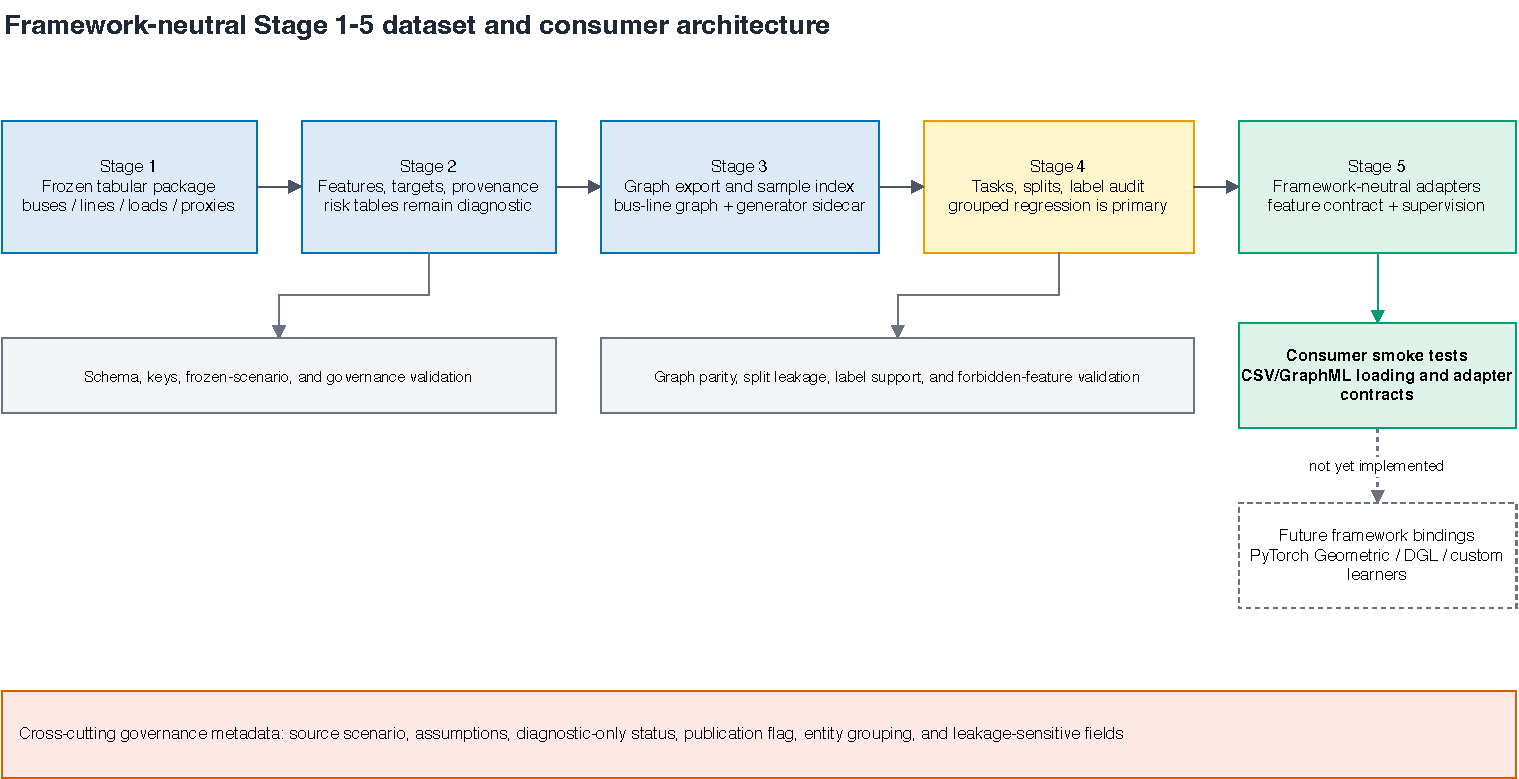
\includegraphics[width=\textwidth]{fig6_dataset_architecture.pdf}
  \caption{Release organization from core topology outputs to staged derivative interfaces. Each stage adds a consumer-facing contract while retaining provenance, diagnostic status, split-control, and publication metadata. Framework-specific tensor bindings remain outside the current release scope.}
  \label{fig:stages}
\end{figure}

\subsection{Released artifacts}

\begin{table}[t]
\centering
\small
\caption{Principal released artifacts described in the manuscript. Additional field-level definitions should be provided in a supplement or archive datasheet.}
\label{tab:composition}
\begin{tabular}{p{0.30\textwidth}rp{0.42\textwidth}}
\toprule
Artifact & Rows/items & Purpose \\
\midrule
Retained candidate branches CSV & 358 & Inter-facility candidate branches with endpoint facilities, source identifiers, geometry-derived length, status, and confidence metadata. \\
Circuit-classification ledger CSV & 1,342 & Full retained and downgraded circuit population with terminal structure, conflict flags, and disposition fields. \\
Selected GraphML multigraph & 484 nodes, 358 edges & All-facility candidate graph including isolates under the declared release policy. \\
Reconstruction-sensitivity CSV & 216 & Parameter sweep across facility sets, buffers, snap thresholds, and merge modes. \\
External triangulation CSV/JSON & 358 branch matches & Public-source evidence categories and supporting summaries for retained branches. \\
External-source audit CSV & 4 sources & Roles and branch-truth limitations of E-REDES, REN, ENTSO-E, and OSM/OpenInfraMap sources. \\
Source manifest JSON & 13 & Source dataset identifiers, roles, retrieval checks, and attribution metadata. \\
Stage~1--5 derivative interfaces & multiple tables & Downstream tabular, graph, benchmark, and adapter views derived from the candidate release. \\
\bottomrule
\end{tabular}
\end{table}

\paragraph{Retained candidate branches CSV.}
The retained branch table (\path{data/processed/at_interfacility_candidate_branches.csv}) is the principal branch-level release record. It contains 358 inter-facility candidate branches generated under the selected setting. Each row represents one retained branch candidate and includes generated branch and circuit identifiers, endpoint facility identifiers and labels, voltage and status fields, geometry-derived length, segment count, source-line membership, confidence metadata, and explicit electrical placeholders where values remain unavailable. Lengths are in physical distance units derived from the projected reconstruction geometry. Missing electrical fields remain missing rather than being backfilled with model defaults. Relationships to the ledger and GraphML are mediated by shared identifiers and endpoint facility references.

\paragraph{Circuit-classification ledger CSV.}
The circuit-classification ledger (\path{data/processed/at_circuit_classification.csv}) contains all 1,342 merged circuit candidates, including the 358 retained records and 984 downgraded outcomes. It serves as the complete disposition ledger for the selected reconstruction. Rows include construction-setting identifiers, terminal structure, facility membership, ambiguity and conflict indicators, geometry type, source-line membership, and downgrade classifications such as self-loop, isolated, single-facility, loop, ambiguous, and tap or multi-terminal. This file is essential for reuse because it exposes what was not retained and why.

\paragraph{Reconstruction-sensitivity CSV.}
The sensitivity table (\path{data/processed/at_paper_logic_parameter_sweep.csv}) stores the full 216-setting reconstruction sweep. Each row corresponds to one combination of facility set, facility buffer, endpoint snap threshold, and merge mode, together with retained-branch counts, ambiguity counts, and graph-structure summaries. The table allows users to reproduce the selected setting and to inspect how alternative settings alter yield and fragmentation. It should be version-linked to the selected release manifest so that the chosen operating point remains auditable.

\paragraph{GraphML multigraph.}
The GraphML file (\path{data/processed/at_paper_logic_graph.graphml}) represents the selected all-facility candidate multigraph. It contains 484 facility nodes, 358 multiedges, 170 connected components, a largest component of size 53, 109 isolates, and 28 parallel edges. Nodes correspond to selected facilities under the release isolate policy; edges correspond to retained inter-facility candidates. The GraphML preserves graph structure, node and edge identifiers, and associated metadata needed for downstream graph analyses. Users should treat this artifact as an inferred graph representation of the candidate release, not as a validated physical network model.

\begin{figure}[t]
  \centering
  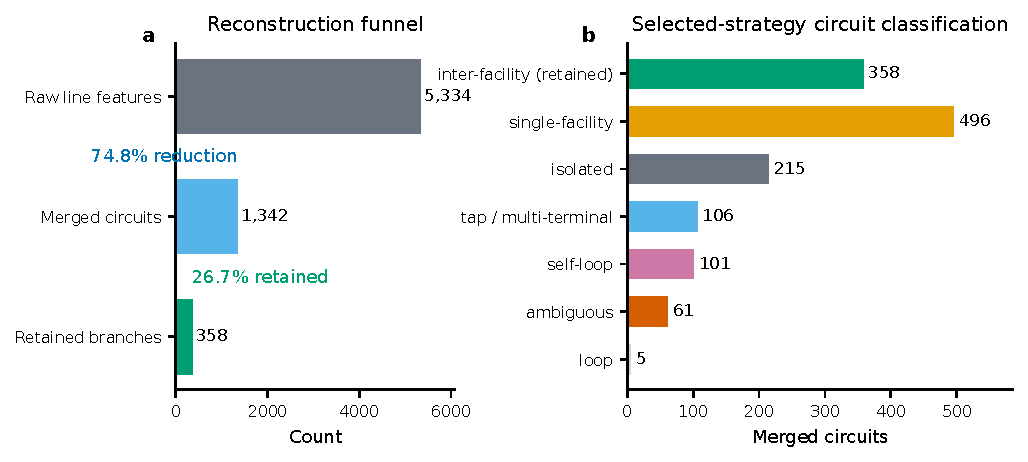
\includegraphics[width=\textwidth]{fig2_reconstruction_funnel.pdf}
  \caption{Record disposition for the selected reconstruction setting. The selected workflow processes 5,334 source line features into 1,342 circuit candidates, retains 358 inter-facility candidate branches, and preserves downgraded classes in the ledger. Retention denotes rule satisfaction under the documented workflow, not operator confirmation.}
  \label{fig:funnel}
\end{figure}

\paragraph{Validation and public-evidence records.}
The validation package includes \path{data/processed/topology_validation/pt_topology_cross_validation_osm_matches.csv}, \path{data/processed/topology_validation/pt_topology_cross_validation_summary.json}, and \path{data/processed/topology_validation/pt_topology_cross_validation_source_audit.csv}. The branch-level table stores the selected public-evidence record, name-match scores, corridor-distance measures, coverage measures, evidence category, and evidence URL for each retained candidate. The source audit distinguishes official consistency sources, transmission-boundary references, and public corridor evidence from branch-level ground truth. No released field is described as a confirmed topology label.

\paragraph{Metadata and manifests.}
The source manifest (\path{data/metadata/reproduction_source_manifest.json}) records source dataset identifiers, source roles, retrieval checks, and attribution metadata for 13 inputs. The release should also include a public-facing manifest or datasheet `[RELEASE DATASHEET NEEDED]` describing file versioning, transformation notices, semantic-status conventions, and archive checksums. This metadata layer is necessary for FAIR-style reuse because many core dataset claims depend on interpretation of provenance and scope, not only on row values.

\paragraph{Optional electrical-readiness records.}
Optional records such as \path{data/processed/at_parameter_feasibility_summary.json}, \path{data/processed/at_line_parameter_inputs.csv}, \path{data/processed/pandapower_schema/pt_schema_summary.json}, and \path{data/processed/acpf_localization/pt_acpf_localization_summary.json} describe electrical-parameter completeness and diagnostic non-convergence boundaries. These files are part of the release because they document what the candidate dataset does \emph{not} yet support. They should be used as readiness diagnostics rather than as evidence that the release constitutes a validated electrical network model.

\paragraph{Stage~1--5 derivative interfaces.}
The Stage~1--5 directories provide frozen tabular views, graph-learning exports, grouped split registries, feature contracts, and framework-neutral adapters. These records document downstream consumption of the candidate topology. In the Scientific Data version of the manuscript, they should be described as derivative interfaces and validation contracts rather than as the primary dataset contribution. A complete archive should include a concise stage inventory and a field-level mapping to the core topology records `[STAGE INTERFACE CROSSWALK NEEDED]`.

\subsection{Detailed structure, fields, and semantics}

The current manuscript can document the main artifacts and their relationships, but a submission-ready archive should provide additional structured tables that are only referenced here as placeholders:
\begin{itemize}
  \item Supplementary Table~S1: complete field-level data dictionary for all released CSV and JSON artifacts `[DATA DICTIONARY / SUPPLEMENT TABLE NEEDED]`;
  \item Supplementary Table~S2: semantic-status and admissibility summary for key columns `[STATUS SEMANTICS SUMMARY TABLE NEEDED]`;
  \item Supplementary Table~S3: archive file inventory with checksums, versions, and MIME types `[ARCHIVE INVENTORY TABLE NEEDED]`.
\end{itemize}

These materials are needed so that a reader can interpret the released records without opening the repository source tree.

\begin{figure}[t]
  \centering
  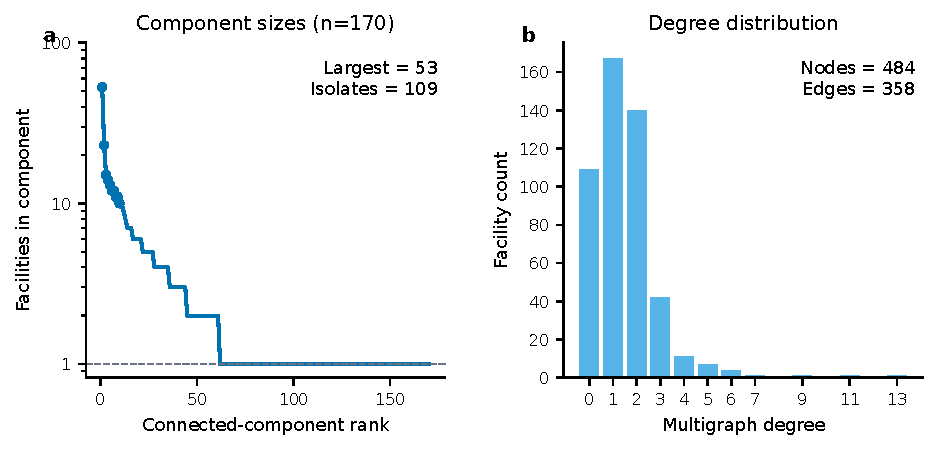
\includegraphics[width=\textwidth]{fig3_topology_quality.pdf}
  \caption{Aggregate structure of the selected all-facility candidate multigraph. Component sizes are shown on a logarithmic vertical scale and the degree histogram retains parallel edges. The figure describes the released graph artifact rather than the physical Portuguese network.}
  \label{fig:topology-quality}
\end{figure}

\section{Technical Validation}

\subsection{Internal validation}

The workflow applies fail-closed checks throughout acquisition, reconstruction, packaging, and staged release. These checks include geometry-type and geometry-validity screening, coordinate-reference handling, endpoint completeness, facility-membership ambiguity, endpoint-cluster composition, mixed voltage or status conflicts, terminal-count classification, branch-key uniqueness, graph/table parity, schema coverage, feature-role constraints, grouped split rules, and forbidden target-derived feature rules in derivative interfaces.

The same validation philosophy extends to the Stage~1--5 derivative artifacts. Structural validators and consumer smoke tests currently pass locally for these downstream interfaces, indicating that the released contracts remain machine-readable and internally consistent. These results support internal usability of the records, but they do not constitute external topology or electrical validation.

\subsection{Structural validation}

Structural validation focuses on whether the reconstructed records satisfy the declared topology-building rules. Under the selected setting, the workflow converts 5,334 line features into 1,342 merged circuit candidates, of which 358 are retained and 984 are downgraded. The downgraded outcomes comprise 496 single-facility records, 215 isolated records, 106 tap or multi-terminal records, 101 self-loops, 61 ambiguous records, and five loop records for the current snapshot. Preservation of these downgraded classes is itself a validation feature because it prevents silent loss of evidence about reconstruction uncertainty.

\subsection{Schema validation}

The release validates that required files, columns, and machine-readable summaries exist and remain aligned across release surfaces. In derivative interfaces, feature contracts and preprocessing contracts also constrain which fields may be used as model inputs and which serve only as labels, split controls, or provenance metadata. This schema-level validation is particularly important because the release includes both core topology records and optional diagnostic layers with different admissible uses.

For the frozen public-validation route, the internal validation export records 25 machine-readable checks across source geometry parsing, retained-branch completeness, ledger accounting, endpoint summaries, facility footprints, GraphML/table parity, sensitivity rows, and artifact hashes. The current result is \status{PASS\_WITH\_WARNINGS}: 23 checks pass and two checks are warnings rather than data-consistency failures. The warnings record that the exact source/release CRS still needs final Data Records wording and that current core artifact hashes are a deterministic baseline for the later clean-room reproduction step. The same export records 5,334 valid source geometries and zero invalid/dropped geometries; zero missing required retained-branch fields; zero missing required ledger fields; 358 retained branches; 984 downgraded or rejected records; 1,342 ledger rows; 64,008 endpoint-index rows across six snap thresholds; and 216 sensitivity rows.

\subsection{Referential integrity}

Referential checks confirm that endpoint facility references, graph node identifiers, staged supervision links, and manifest-linked artifact relationships resolve to valid upstream records. In the selected release, graph and table views are checked for parity so that counts in the GraphML, retained branch table, and selected facility set remain consistent with the documented isolate policy. The same referential logic is used in staged derivative exports so that downstream interfaces cannot silently point to missing topology objects.

\subsection{Graph consistency}

The selected all-facility graph contains 484 facilities, 358 multiedges, 170 connected components, a largest component of size 53, 109 isolates, and 28 parallel edges. The edge-induced graph contains 375 incident facilities, while the all-facility GraphML additionally preserves selected isolates. This accounting distinction is stored explicitly because graph artifacts with different isolate policies can otherwise appear inconsistent. Graph-level summaries therefore validate the released artifact against its own declared representation rather than against an external ground-truth network.

The GraphML/table parity check confirms that all 358 retained branch identifiers appear as GraphML edge identifiers, that no extra GraphML branch identifiers are present, and that every retained branch endpoint facility resolves to a GraphML node. The GraphML has 27 parallel facility pairs, 55 edge records participating in parallel pairs, and 28 extra parallel-edge records beyond one edge per facility pair. The missingness export also confirms that all retained-branch electrical fields \code{r}, \code{x}, \code{b}, thermal limits, transformer impedance, and tap settings remain explicitly marked as \status{MISSING\_NOT\_ESTIMATED}; these missing values are part of the release semantics rather than silent nulls.

\subsection{Sensitivity analysis}

Sensitivity analysis addresses whether the selected release point is stable under the declared reconstruction design space. The direct endpoint-to-substation baseline yields 51 merged edges and a six-node largest component, whereas the selected reconstruction yields 358 retained edges and a 53-node largest component for the current snapshot. These values describe yield and connectivity under two workflows; they are not treated as external accuracy improvements.

Across the 216-setting sweep, increasing the facility buffer from 100~m to 500~m at a 0.5~m endpoint snap threshold raises retained branches from 358 to 369 but also increases ambiguity from 61 to 89 and reduces the largest component from 53 to 27. At 50~m endpoint snapping, only three inter-facility circuits remain for each tested buffer. These results support the claim that reconstruction outputs are sensitive to plausible preprocessing settings and that the selected operating point is a documented trade-off rather than a uniquely correct solution.

\begin{figure}[t]
  \centering
  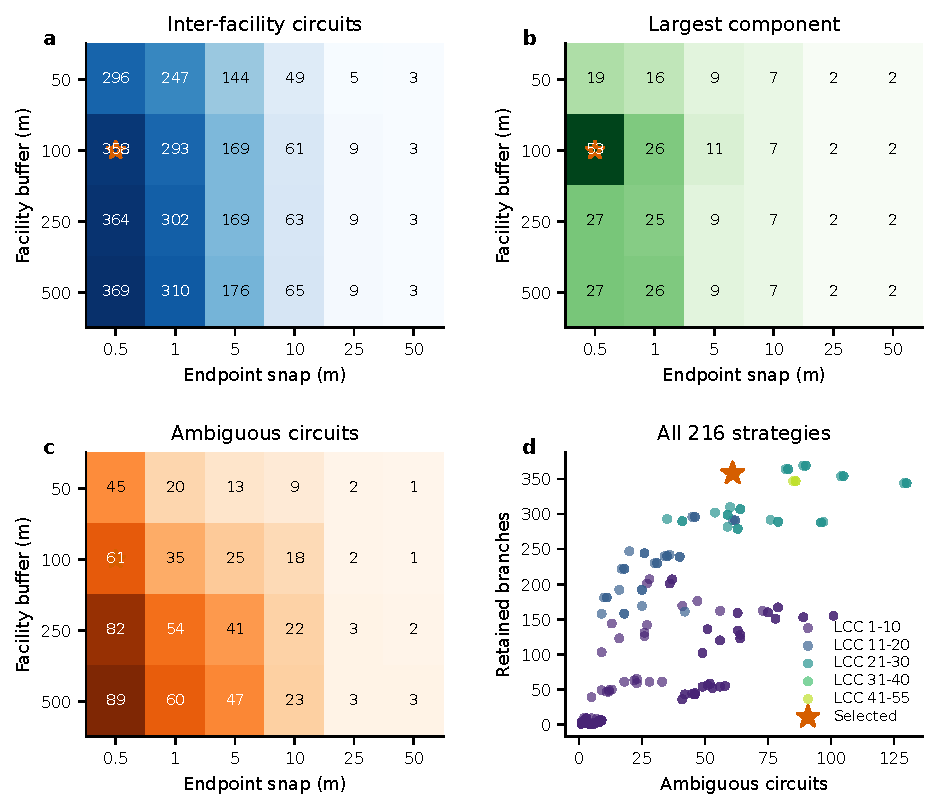
\includegraphics[width=\textwidth]{fig4_sensitivity_analysis.pdf}
  \caption{Sensitivity of retained-branch counts, ambiguity, and graph connectivity to facility buffers and endpoint snap thresholds. The marked operating point indicates the documented selected setting for the release; it is not an externally calibrated optimum.}
  \label{fig:sensitivity}
\end{figure}

\subsection{External triangulation}

The external triangulation workflow searches for branch-level public evidence outside the selected reconstruction rule. The current implementation uses \osminfra 60~kV \code{power=line} and \code{power=cable} records in Portugal, caches the raw Overpass response, parses voltage, operator, name, reference, circuit, and geometry fields, and compares each retained branch against these public records by endpoint-name overlap and corridor proximity.

\begin{table}[t]
\centering
\small
\caption{\osminfra public-source triangulation for the 358 retained candidate branches. Categories describe review-prioritization evidence, not truth labels.}
\label{tab:osm-triangulation}
\begin{tabular}{p{0.46\textwidth}rp{0.32\textwidth}}
\toprule
Evidence category & Branches & Interpretation \\
\midrule
\status{OSM\_NAME\_OPERATOR\_STRONG} & 183 & Endpoint names appear in a 60~kV E-REDES-labelled OSM record. \\
\status{OSM\_GEOMETRY\_OPERATOR\_STRONG} & 64 & Candidate corridor is close to a 60~kV E-REDES-labelled OSM corridor. \\
\status{OSM\_PARTIAL\_NAME\_NEARBY} & 56 & One endpoint name appears and a nearby 60~kV corridor is present. \\
\status{OSM\_GEOMETRY\_MEDIUM} & 48 & Candidate overlaps a 60~kV public corridor without strong name evidence. \\
\status{OSM\_NEARBY\_WEAK} & 7 & A nearby 60~kV public feature is present, but evidence is incomplete. \\
\status{NO\_EXTERNAL\_OSM\_MATCH} & 0 & No retained branch falls in this class for the documented snapshot. \\
\bottomrule
\end{tabular}
\end{table}

For the current snapshot, 5,551 Portuguese 60~kV public ways are cached and all 358 retained candidate branches receive a non-empty public-evidence category, with 247 strong, 104 medium, and seven weak matches. This result provides public-source concordance and a branch-level evidence index. It does not establish operator validation or branch accuracy, because OSM coverage and tagging are non-authoritative. To audit provenance risk, the release records current OSM metadata for the 5,551 cached public ways and full version histories for the 271 unique OSM ways matched to retained branches, covering 2,326 historical versions. The branch-level audit classifies 266 retained branches as having stronger inspectable public evidence, 87 as unknown independence, and five as possibly same-source or operator-tag-only evidence. These categories distinguish public concordance from more inspectable public corroboration, but they still must not be interpreted as precision, recall, or confirmation of every retained branch.

\ifdefined\PTPublicValidationOnly
\subsection{Validation strategy without independent human adjudication}

This release does not use dual independent human review as a validation layer and does not report a human-adjudicated accuracy metric. Instead, the validation argument is deliberately claim-bounded. Internal tests establish that the released records satisfy their declared schema, classification, provenance, and graph contracts. The 216-setting sweep quantifies sensitivity to reconstruction choices. The external comparison records concordance with a separately maintained public geospatial layer while preserving the evidence category and source caveat for every retained branch. Together, these tests support reproducibility, internal consistency, sensitivity transparency, and public-source triangulation; they do not support a claim that the inferred connections reproduce the operator's true network.

The public-source comparison is evaluated at branch level but is not converted into binary ground truth. Consequently, the manuscript reports category counts and matching variables rather than precision, recall, $F_1$, or confidence intervals. Precision is not independently estimated, and national or real-network recall is not estimable because neither an authoritative branch census nor a probability sample of true Portuguese 60~kV connections is available.

\begin{table}[t]
\centering
\small
\caption{Claim-bounded validation used in the public-source validation route. ``Supported'' refers to the stated dataset property, not to physical topology truth.}
\label{tab:claim-bounded-validation}
\begin{tabular}{p{0.31\textwidth}p{0.27\textwidth}p{0.31\textwidth}}
\toprule
Validation layer & Supported interpretation & Interpretation explicitly excluded \\
\midrule
Geometry, CRS, schema, and key checks & Machine-readable and internally coherent release & Correct physical connectivity \\
Ledger and graph/table parity & Complete accounting under declared rules & Completeness of the real grid \\
216-setting sensitivity sweep & Dependence on documented reconstruction choices & Externally optimal parameter setting \\
OSM/OpenInfraMap triangulation & Public-source name and corridor concordance & Operator validation or statistical accuracy \\
Electrical-readiness gates & Explicit identification of missing or diagnostic fields & AC power-flow or operational readiness \\
\bottomrule
\end{tabular}
\end{table}

Two deterministic negative controls test whether the public-source matcher responds to deliberately broken evidence channels. First, an endpoint-name control was run on all 358 retained branches. The control keeps each branch geometry, voltage, status, length, confidence score, and branch identifier fixed, but replaces the endpoint-name pair with a length-stratified cyclic shift from another retained branch using seed 20260714. Under the unmodified endpoint names, 183 of 358 branches receive strong name-based OSM/OpenInfraMap evidence. Under corrupted endpoint names, this falls to 9 of 358 branches, a 95.1\% relative reduction. Second, a spatial-alignment control keeps endpoint names and tabular branch attributes fixed but translates every branch geometry by +1.75 degrees longitude and +0.85 degrees latitude. All 358 transformed geometries remain valid and no records are excluded after transformation. Under the unmodified geometries, 290 of 358 branches satisfy the corridor-evidence criterion; under displaced geometries, this falls to 1 of 358 branches, a 99.7\% relative reduction. These controls support the selectivity of the endpoint-name and corridor components of the matcher. They do not estimate topology accuracy, precision, recall, or operator validation.
\else
\subsection{Manual validation protocol}

The manual validation workflow is defined but not yet complete. A deterministic proportional sample selects 100 of the 358 retained candidate branches across 27 strata defined by confidence band, component role, asset type, and parallel-edge context. Two independent reviews are allocated per sampled branch. Each review must cite operator or other inspectable evidence, record confirm, reject, or uncertain status, and state reviewer confidence. Disagreements are expected to be resolved by adjudication.

\begin{table}[t]
\centering
\small
\caption{Current manual-validation status. Quantities shown here describe protocol state rather than measured accuracy.}
\label{tab:external-validation}
\begin{tabular}{lr}
\toprule
Item & Current value \\
\midrule
Candidate-branch population & 358 \\
\osminfra 60~kV ways cached & 5,551 \\
Branches with non-empty public evidence & 358 \\
Strong public evidence branches & 247 \\
Medium public evidence branches & 104 \\
Weak public evidence branches & 7 \\
Stratified review sample & 100 \\
Planned independent reviews & 200 \\
Adjudicated branches & 0 \\
Unresolved branches & 100 \\
Precision estimate & \status{not evaluable} \\
Recall estimate & \status{not estimable from retained-only sample} \\
\bottomrule
\end{tabular}
\end{table}

After at least 50 branches receive two evidence-complete reviews and adjudication, the summarizer can report unweighted and sampling-weighted precision with Wilson 95\% intervals and disagreement counts. A separate rejected or downgraded sample is required before recall can be estimated. These outputs should be added before submission if the paper is to report branch-accuracy metrics `[ADJUDICATED VALIDATION RESULTS NEEDED]`.
\fi

\subsection{Validation boundaries}

The current validation evidence supports internal consistency, release transparency, sensitivity analysis, and public-source triangulation. It does not support claims of operator-confirmed topology accuracy, independently estimated branch precision, national-grid recall or completeness, or electrical-operating realism. Optional electrical-readiness artifacts remain diagnostic because branch-specific parameters, transformer details, control states, measured injections, and verified boundaries are incomplete or scenario-derived. The full diagnostic AC power-flow extension therefore remains outside the validated core dataset and should not be used to imply AC power-flow or OPF readiness.

\FloatBarrier
\section{Usage Notes}

\subsection{Intended uses}

The core release is intended for topology-reconstruction studies, geospatial data integration, provenance-aware network analysis, uncertainty analysis, dataset-engineering experiments, and development of downstream graph or tabular interfaces that preserve release semantics. The retained branch table and circuit-classification ledger should be used together whenever a study depends on understanding what was retained, what was downgraded, and why.

\subsection{Non-intended uses}

The release is not intended for operational switching studies, protection analysis, security assessment, contingency analysis, congestion forecasting, infrastructure-targeting applications, emergency operations, asset-condition assessment, commercial network-capacity claims, regulatory network-capacity claims, or claims about the actual Portuguese grid. The candidate topology should not be described as operator-validated, and the optional diagnostic electrical and learning layers should not be described as measured system behavior.

\subsection{Reading provenance and semantic status fields}

Users should read semantic status fields before aggregating or modeling the records. Observed, derived, inferred, source-backed, scenario-assumed, benchmark-only, proxy, and missing fields represent distinct evidence types. Studies that require source-backed physical parameters or operator-confirmed connectivity should filter the release accordingly and should not treat inferred or scenario-derived fields as interchangeable with observations.

\subsection{How to use GraphML}

The GraphML is the most direct representation of the released candidate multigraph for graph analysis. It preserves the selected all-facility node set, including isolates, and therefore aligns with the documented component and degree summaries. Users comparing the GraphML with edge-induced views should account for the explicit isolate policy. Parallel edges are part of the released graph structure and should not be collapsed without documenting the transformation.

\subsection{How to use CSV records}

The retained candidate branch CSV is the preferred branch-level topology table. The circuit-classification ledger should be consulted whenever a downstream workflow depends on failure modes, ambiguity, or alternative selection rules. Validation CSV and JSON records document evidence categories, sampling strata, and release-manifest relationships. Stage~1--5 derivative CSV outputs should be treated as consumer-facing views of the candidate resource rather than replacements for the core topology records.

\subsection{Limitations}

The release has four main limitations. First, it is a candidate topology derived from public E-REDES records rather than an operator-confirmed network model. Second, external triangulation provides public-source concordance categories rather than truth labels: precision is not independently estimated, and national or real-network recall cannot be estimated from the available records. Third, electrical parameters, transformer details, operating controls, and injections are incomplete, missing, or scenario-derived in the optional electrical extension. Fourth, downstream labels and baselines in the staged derivative interfaces are diagnostic and should be interpreted as interface checks rather than validated operational targets.

\begin{figure}[t]
  \centering
  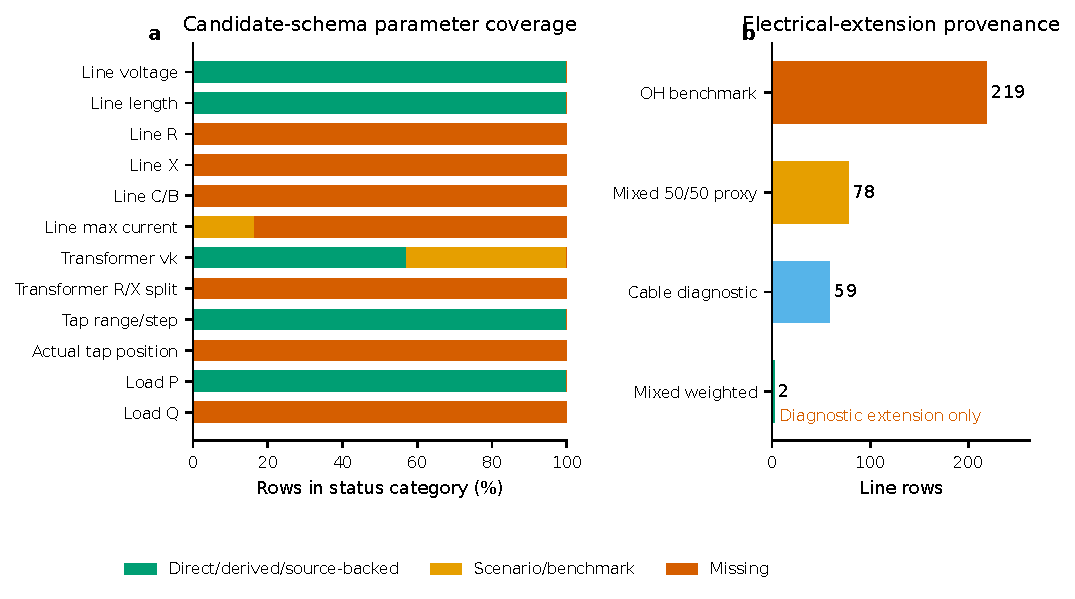
\includegraphics[width=\textwidth]{fig5_parameter_coverage.pdf}
  \caption{Coverage and provenance categories in the optional electrical extension. Topology-derived and source-backed fields remain separate from scenario, benchmark, proxy, and missing values so that reuse boundaries are explicit.}
  \label{fig:parameters}
\end{figure}

\section*{Data Availability}

The dataset described here should be released as a versioned archive containing the core topology records, validation outputs, provenance metadata, a field-level data dictionary, and a checksum-linked manifest. Archive identifiers are still pending and should be inserted as `[DATASET DOI NEEDED]`, `[VERSIONED ARCHIVE URL NEEDED]`, and `[RELEASE VERSION NEEDED]`. The archive should preserve the E-REDES attribution text, portal URL, source dataset identifiers, access dates, CC BY~4.0 reference, and an indication of modifications. If some derivative artifacts are excluded from the public package, the final archive should document those omissions explicitly `[PUBLIC ARCHIVE CONTENT NOTE NEEDED]`.

\section*{Code Availability}

The reconstruction, validation, and figure-generation code is maintained in the \project repository and should be cited as a versioned release rather than as a moving branch. The repository URL and release tag should be inserted as `[CODE REPOSITORY URL NEEDED]` and `[CODE RELEASE TAG OR COMMIT NEEDED]`. The code remains MIT-licensed. This code license applies to software only and does not replace the attribution and modification requirements attached to E-REDES-derived data artifacts.

\section*{Author Contributions}

`[AUTHOR CONTRIBUTIONS NEEDED]`

\section*{Acknowledgements}

`[ACKNOWLEDGEMENTS NEEDED]`

\section*{Funding}

`[FUNDING STATEMENT NEEDED]`

\section*{Competing Interests}

The author(s) declare `[COMPETING INTERESTS STATEMENT NEEDED]`.

\bibliographystyle{plainnat}
\bibliography{references}

\end{document}
